%--------------------------------------------------------------------------
\chapter{\label{Appendix_A}Computational Details}
%--------------------------------------------------------------------------

%--------------------------------------------------------------------------
\section{\label{Appendix_A:Derivation}
Derivation of Phonon Spectral Energy Density, $\Phi$}
%--------------------------------------------------------------------------

To derive the correct expression for the phonon SED, $\Phi$, we begin 
with harmonic lattice dynamics theory.\cite{wallace_thermodynamics_1972,
dove_introduction_1993} In reciprocal space, the system Hamiltonian, 
$H$, is
\begin{equation}\label{E:H_HLD}
\begin{split}
H=&\frac{1}{2}\SUM{}{}\left[\dot{q}^*\kvt \dot{q}\kvt + \omega_0^2\kv 
q^*\kvt q\kvt\right]\\
 =&\SUM{}{}\left[T\kvt + V\kvt\right],
\end{split}
\end{equation}
where $t$ is time, $\omega_0\kv$ is the frequency of the phonon mode 
denoted by
wave vector $\pmb{\kappa}$ and dispersion branch $\nu$, and $N$ and 
$n$ are
the total number of unit cells and the number of atoms in the unit cell.
The
Hamiltonian is the total system energy and is the sum of the mode- and
time-dependent kinetic and potential energies, $T\kvt$ and $V\kvt$.  The
phonon normal mode coordinate, $q\kvt$ and its time derivative, 
$q\kvt$, are given by
\begin{equation}\label{A:E:q_HLD}
\begin{split}
q\kvt=&\SUM{0}{}\sqrt{\frac{m_b}{N}}u_{\alpha}\lbt e^*\kvba
\EXP{i\pmb{\kappa}\cdot\mathbf{r}_0\ab{l}{0}}
\end{split}
\end{equation}
and
\begin{equation}\label{A:E:qdot_HLD}
\begin{split}
\dot{q}\kvt{}{}{}=&\SUM{0}{}\sqrt{\frac{m_b}{N}}\dot{u}_{\alpha}\lbt
e^*\kvba\EXP{i\pmb{\kappa}\cdot\mathbf{r}_0\ab{l}{0}},
\end{split}
\end{equation}
where $m_b$ is the mass of the $b^{\textrm{th}}$ atom in the unit 
cell and
$\mathbf{r}_0\ab{l}{0}$ is the equilibrium position vector of the
$l^{\textrm{th}}$ unit cell. The $\alpha$-component of the displacement 
from
equilibrium, $u_{\alpha}\lbt$, and velocity, $\dot{u}_{\alpha}\lbt$, 
of the
$b^{\textrm{th}}$ atom in the $l^{\textrm{th}}$ unit cell are 
time-dependent
and are related to the phonon mode coordinates through the 
time-independent
eigenvector that has components $e\kvba$. 

The potential and kinetic energies of the normal mode are
\begin{equation}\label{A:E:q_U}
\begin{split}
V\kvt = \frac{1}{2} \omega \kv^2 q^*\kvt q\kvt
\end{split}
\end{equation}
and
\begin{equation}\label{A:E:q_T}
\begin{split}
T\kvt = \frac{1}{2} \dot{q}^*\kvt \dot{q}\kvt, 
\end{split}
\end{equation}
such that the total energy of the normal mode is
\begin{equation}\label{A:E:q_E}
\begin{split}
E\kvt = T\kvt + V\kvt.
\end{split}
\end{equation}
In an anharmonic system, the phonon populations fluctuate about the
equilibrium distribution function.\cite{wallace_thermodynamics_1972,
maradudin_dynamical_1974,srivastava_physics_1990} 
The phonon mode 
coordinate for the mode described by ($\pmb{\kappa},\nu$) and its time
derivative can be written as
\begin{equation}\label{A:E:q_A}
\begin{split}
q\kvt=&q_{SS}\kvt+q_{T}\kvt
\end{split}
\end{equation}
and
\begin{equation}\label{A:E:qdot_A}
\begin{split}
\dot{q}\kvt=& \dot{q}_{SS}\kvt+\dot{q}_{T}\kvt.
\end{split}
\end{equation}
The steady-state ($SS$) and transient ($T$) parts and their time 
derivatives are given by
\begin{equation}\label{A:E:q_A_SS}
\begin{split}
q_{SS}\kvt=& C_1\kv\exp[i\omega_0\kv t]
\\& +C_2\kv\exp[-i\omega_0\kv t],
\end{split}
\end{equation}
\begin{equation}\label{A:E:q_A_T}
\begin{split}
q_{T}\kvt=& \EXP{-\Gamma\kv |t|}\lbrace C_3\kv\EXP{i\omega_0\kv t}
\\ &-C_4\kv\EXP{-i\omega_0\kv t } \rbrace,
\end{split}
\end{equation}
\begin{equation}\label{A:E:qdot_A_SS}
\begin{split}
\dot{q}_{SS}\kvt=& i\omega_0\left\{C_1\kv\exp[i\omega_0\kv t]-C_2\kv
\exp[-i\omega_0\kv t]\right\} ,
\end{split}
\end{equation}
and
\begin{equation}\label{E:qdot_A_T}
\begin{split}
\dot{q}_{T}\kvt=& \EXP{-\Gamma\kv |t|}\left\{C_3\kv
\left[i\omega_0\kv-\Gamma\kv\right]\EXP{i\omega_0\kv t}\right. \\
& \left.-C_4\kv\left[i\omega_0\kv+\Gamma\kv\right]\EXP{-i\omega_0\kv t}\;
\right\},
\end{split}
\end{equation}
where the $C$s are constants and $\omega_0\kv$ and $\Gamma\kv$ are the 
phonon
mode frequency and linewidth.  The transient part
describes the creation of an excess in the population of a phonon mode 
for
$t<0$ and its decay back to equilibrium for $t>0$.

Phonon population fluctuations are commonly modeled using the excitation 
and decay of
a single phonon mode (i.e., the single mode relaxation time approximation).
In a real system, there will be multiple phonons in
each mode that simultaneously grow or decay with time.  Thus, dealing 
only
with $\dot{q}$, we let
\begin{equation}\label{A:E:qdot_A_kvbat}
\begin{split}
\dot{q}\kvt =& \sum_j i\EXP{-\Gamma\kv |t-t_j|}\times \\
& \lbrace A_j\kv\left[\omega_0\kv+i\Gamma\kv\right]
\EXP{i\omega_0\kv (t-t_j)} \\
& -B_j\kv \left[\omega_0\kv-i\Gamma\kv\right]\EXP{-i\omega_0\kv (t-t_j) }
\; \rbrace,
\end{split}
\end{equation}
where many phonons in each mode, indexed by $j$, are simultaneously 
being
created and destroyed.  The phonons grow for $t<t_j$, decay for $t>t_j$,
and $A_j$ and $B_j$ are constants.  We are  not concerned with the 
values of
$t_j$, $A_j$, and $B_j$, though they should satisfy the long-time average
$\langle\dot{q}^*\kvt\dot{q}\kvt\rangle = \langle\dot{q}_{SS}^*\kvt
\dot{q}_{SS}\kvt\rangle$.

The expectation value of the kinetic energy of the normal mode in the time 
domain is
\begin{equation}\label{A:E:ave_T_t}
\begin{split}
\langle T\kv \rangle=&\frac{1}{2}\lim_{\tau_0\rightarrow\infty}
\frac{1}{\tau_0}\int_{0}^{\tau_0}\dot{q}^*\kvt\dot{q}\kvt dt.
\end{split}
\end{equation}
The expectation value of the kinetic energy of the normal mode can 
be transformed from the time domain to the
frequency domain by Parseval's theorem,\cite{rudin_real_1987} giving
\begin{equation}\label{A:E:ave_T_w1}
\begin{split}
T\kvw=&\lim_{\tau_0\rightarrow\infty}\frac{1}{2\tau_0}
\left|\frac{1}{\sqrt{2\pi}}\int_{0}^{\tau_0}\dot{q}\kvt
\exp(-i\omega t)dt\right|^2.
\end{split}
\end{equation}
By substituting Eq$.$ \eqref{A:E:qdot_A_kvbat} into Eq$.$ 
\eqref{A:E:ave_T_w1} and performing the time integration we find
\begin{equation}\label{A:E:ave_T_w_int}
\begin{split}
T\kvw = \frac{1}{16\pi\tau_0}\left|\sum_j\EXP{-i\omega t_j} 
\left\{A_j\kv\frac{\omega_0\kv+i\Gamma\kv}{\omega_0\kv-\omega+i\Gamma\kv}
\right.\right.\\
\left.\left.+B_j\kv\frac{\omega_0\kv-i\Gamma\kv}
{\omega_0\kv+\omega-i\Gamma\kv}\right\}\right|^2.
\end{split}
\end{equation}
We are primarily interested in values of $\omega$ where 
$\omega\approx\omega_0$ when $\Gamma<<\omega_0$.  
When $\omega\approx\omega_0$, 
the term involving $A_j$ becomes large and the term involving $B_j$ can 
be neglected (alternatively, we could ignore the term involving $A_j$ 
when $\omega\approx-\omega_0$).  Hence, we find
\begin{equation}\label{A:E:ave_T_w_approx}
\begin{split}
T\kvw=\frac{1}{16\pi\tau_0}\sum_j\sum_{j'}\cos\left[\omega (t_{j'}-t_j)
\right]A_j\kv A_{j'}\kv\\
\times\frac{\omega_0^2\kv+\Gamma^2\kv}{\Gamma\kv}\frac{\Gamma\kv}
{[\omega_0\kv-\omega]^2+\Gamma^2\kv}.
\end{split}
\end{equation}
We arrive at the expression for the phonon spectral energy density for the 
wavevector $\pmb{\kappa}$ by summing Eq$.$ \eqref{A:E:ave_T_w_approx} 
over the different polarizations $\nu$,
\begin{equation}\label{A:E:Lorentzian_NMD}
\begin{split}
\Phi(\pmb{\kappa},\omega) = 2\sum_{\nu}^{3n} T\kvw=\sum_{\nu}^{3n}C_0\kv
\frac{\Gamma\kv/\pi}{[\omega_0\kv-\omega]^2+\Gamma^2\kv},
\end{split}
\end{equation}
where the factor of two comes from equipartition of kinetic and potential 
energy (valid for a harmonic classical system, see Section 
\ref{Subsection_Comp_Details_3}), and
\begin{equation}\label{A:E:C_0}
\begin{split}
C_0\kv = \sum_j\sum_{j'}\cos\left[\omega (t_{j'}-t_j)\right]A_j\kv A_{j'}
\kv\frac{\omega_0^2\kv+\Gamma^2\kv}{8\tau_0\Gamma\kv}.
\end{split}
\end{equation}
Thus, the phonon spectral energy density $\Phi(\pmb{\kappa},\omega)$ is 
a superposition of $3n$ Lorentzian
functions with centers at $\omega_0\kv$ (one for each polarization) with 
a linewidth (half-width at half-maximum) of
$\Gamma\kv$. $\Phi$ is a spectral energy density since its integral over 
all wavevectors and frequencies is the total crystal energy, i.e., 
the Hamiltonian is
\begin{equation}\label{A:E:equipartition}
\begin{split}
H=\int\limits_{V_{BZ}} \int_{0}^{\infty}\Phi(\pmb{\kappa},\omega)d\omega 
d\pmb{\kappa},
\end{split}
\end{equation}
where $V_{BZ}$ is the volume of the first Brillouin zone.  Like the 
frequency broadening, there is also a broadening of the SED in wavevector.
\cite{turney_predicting_2009-1} For a finite sampling of the 
first Brillouin zone, 
the Hamiltonian can be approximated by
\begin{equation}\label{A:E:equipartition}
\begin{split}
H \approx 2\sum_{\pmb{\kappa},\nu}^{N,3n}\langle T\kvt\rangle = 
\sum_{\pmb{\kappa}}^N \int_{0}^{\infty}\Phi(\omega,\pmb{\kappa})d\omega.
\end{split}
\end{equation}


%--------------------------------------------------------------------------
\section{\label{Appendix_B}Interpretation of $\Phi'$}
%--------------------------------------------------------------------------

As demonstrated in Section \ref{S:Subsection_prop_LJ}, $\Phi'$ is not 
the phonon spectral energy density, $\Phi$, defined by Eq$.$ 
\eqref{E:Lorentzian_NMD_fft}. Our findings and those of others,
\cite{maruyama_molecular_2003,koker_thermal_2009,
thomas_predicting_2010,qiu_molecular_2011,shiomi_thermal_2011} 
however, suggest that $\Phi'$ does contain accurate information about 
the phonon frequencies. To understand this expression, we start with 
the real-space atomic velocities as 
represented by the normal mode velocities, $\dot{q}\kpvt$ 
\cite{dove_introduction_1993},
\begin{equation}\label{E:udot_HLD}
\begin{split}
\dot{u}_{\alpha}\lbt = &\SUMprime{2}{} \frac{1}{\sqrt{m_bN}} 
\EXP{i\pmb{\kappa}^{'}\cdot\mathbf{r}_0\ab{l}{0}} e^*\kpvba 
\dot{q}\kpvt{}{}{}.
\end{split}
\end{equation}
Fourier transforming both sides of Equation \eqref{E:udot_HLD} in time 
and space, taking the complex modulus, and summing over the atoms in 
the unit cell 
and the Cartesian directions yields
\begin{equation}\label{SED}
\begin{split}
\lim_{\tau_0\rightarrow\infty}\frac{1}{4\pi\tau_0} \sum_\alpha^3 
\sum_b^n \frac{m_b}{N} 
\left\lvert \sum_l^N  \int_{0}^{\tau_0} \dot{u}_{\alpha}\lbt 
\EXP{\Theta} dt \right\rvert^2 =
\\ \lim_{\tau_0\rightarrow\infty}\frac{1}{4\pi\tau_0} \sum_\alpha^3 
\sum_b^n 
\left\lvert \frac{m_b^{3/2}}{\sqrt{N}} \sum_l^N \sum_{\nu}^{3n} e^*\kvba 
\int_{0}^{\tau_0}\dot{q}\kvt\EXP{\Theta}dt \right\rvert^2 ,
\end{split}
\end{equation}
where the the sum over $\pmb{\kappa}^{'}$ on the right-hand-side is 
reduced to a 
single wavevector by the orthogonality of the allowed wavevectors over 
the periodic 
domain. Equation \eqref{Lorentzian_SED} is the finite integration of the 
left-hand-side of Eq. \eqref{SED}.

Under the harmonic approximation, the phonons 
are non-interacting and have no transient response beyond a harmonic 
oscillation [see Appendix \ref{Appendix_A:Derivation},  
Eqs$.$ \eqref{A:E:qdot_A} and \eqref{E:qdot_A_T}],
\begin{equation}\label{E:qdot_A_SS}
\begin{split}
\dot{q}\kvt =& \dot{q}_{SS}\kvt  \\
=& i\omega_0\kv\left\{C_1\kv\exp[i\omega_0\kv t]-C_2\kv
\exp[-i\omega_0\kv t]\right\}.
 \end{split}
\end{equation}
Inserting Eq$.$ \eqref{E:qdot_A_SS} into the right hand side of Eq$.$ 
\eqref{SED} gives
\begin{equation}\label{Delta_SED}
\begin{split}
\sum_\alpha^3 \sum_b^n m_b \left| \sum_l^N  \int_{-\infty}^{\infty} 
\dot{u}_{\alpha}\lbt \EXP{i\pmb{\kappa}\cdot
\mathbf{r}_0\ab{l}{0}-i\omega t} 
dt \right|^2 =& \\
\sum_\alpha^3 \sum_b^n\left| \frac{m_b^{3/2}}{\sqrt{N}} \sum_l^N 
\sum_{\nu}^{3n}  D\kvba \EXP{i\pmb{\kappa}\cdot\mathbf{r}_0\ab{l}{0}} 
\delta[ \omega_0\kv - \omega] \right|^2 ,
 \end{split}
\end{equation}
where $D\kvba = i\sqrt{2\pi} \omega_0\kv C_1\kv e^*\kvba$, $\delta$ is 
the Dirac function, and values of $\omega \le 0$ are ignored. Thus, at 
zero temperature Eq$.$ \eqref{Lorentzian_SED} is a superposition of Dirac 
functions at the phonon frequencies $\omega_0\kv$.

Equation \eqref{Lorentzian_SED} is similar to the definition of 
the displacement structure factor
\cite{volz_molecular-dynamics_2000,horbach_high_2001,
martin-mayor_dynamical_2001,christie_vibrational_2007,
beltukov_ioffe-regel_2013}
\begin{equation}\label{Dynam_SF}
\begin{split}
S_{D}(\pmb{\kappa},\omega) = & \frac{1}{4\pi\tau_0} \left| \sum_\alpha^3 
\sum_b^n \frac{m_b}{N}
 \sum_l^N  \int_{0}^{\tau_0} \dot{u}_{\alpha}\lbt \EXP{\Theta} dt 
\right|^2,
\end{split}
\end{equation}
which is related to the static structure factor 
\cite{biswas_vibrational_1988,feldman_thermal_1993,
allen_diffusons_1999,feldman_numerical_1999,
taraskin_determination_1999,taraskin_propagation_2000,
feldman_calculations_2002,ciliberti_brillouin_2003,
shintani_universal_2008,wyart_scaling_2010,
beltukov_ioffe-regel_2013,larkin_predicting_2013,
marruzzo_heterogeneous_2013} (see Sections \ref{S:Dispersion} 
and \ref{S:Structure}). 
\cite{beltukov_ioffe-regel_2013}. The difference between Eqs. 
\eqref{Lorentzian_SED} and \eqref{Dynam_SF} is that the 
summations over $\alpha$ and $b$ occur inside the square modulus 
for Eq. \eqref{Dynam_SF}. With the summations inside the 
square modulus, the orthonormality of the mode eigenvectors 
can be used to show that the static and dynamic 
structure factors are equivalent under the harmonic approximation.
\cite{beltukov_ioffe-regel_2013} 
% The structure factors also obey the sum rule,
% \begin{equation}\label{Delta_SED}
% \begin{split}
% DOS(\omega) = \frac{1}{\pi} \sum_{\pmb{\kappa}}S(\pmb{\kappa},\omega)
% \end{split}
% \end{equation}
% where $DOS(\omega)$ is the normalized vibrational density of states 
% (see Sections \ref{S:VC Gamma DOS} and \ref{FIG:DOS}).
% \ref{beltukov_ioffe-regel_2013}  



% %--------------------------------------------------------------------------
% \section{\label{A:unitcell}Unit Cell and Supercell Representations (WORK)}
% %--------------------------------------------------------------------------
% 
% %--------------------------------------------------------------------------
% \subsection{\label{A:unitcell}Primitive and Conventional 
% Unit Cells (WORK)}
% %--------------------------------------------------------------------------
% 
% Harmonic lattice dynamics is a framework for determining the frequencies 
% and mode shapes of a linear mass-spring system. For a periodic system, 
% the unit cell (i.e., the basis) and lattice vectors are first specified 
% based on the atomic structure. This specification is not unique. For 
% example, as shown in Table \ref{T-unitcell}, one can choose a one 
% atom-basis and a face-centered cubic lattice (the primitive unit cell) 
% or a four-atom basis and the simple cubic lattice (the conventional unit 
% cell) to describe the same structure. The unit cell choice may be related 
% to theoretical or computational complexity, but will not affect the bulk 
% properties (e.g., heat capacity or thermal conductivity).
% 
% 
% 
% The choice of unit cell and supecell size determines the allowed 
% wavevectors of a system (see Section ). 
% The choice of unit cell, however, does not affect the allowed 
% wavevectors, only their representation. 
% 
% Let's use the LJ argon FCC crystal as an example.  The system has a one 
% atom basis with the primitive unit cell. 
% 
% For supercells constructed 
% using the conventional 
% 
% In general, there may not be a mapping There exists a mapping between 
% 
% The code works by recognizing that 
% \href{http://en.wikipedia.org/wiki/Reciprocal_lattice#Face-centered_cubic_.28FCC.29_lattice}
% {the reciprocal space for an FCC lattice is a BCC lattice}. 
% 
% \href{https://github.com/jasonlarkin/disorder/blob/master/matlab/m_lj_prim_conv_mapping.m}
% {lennard-jones FCC primitive conventional mapping}
% 
% Note: this script can be run using the open-source package 
% \href{http://www.gnu.org/software/octave/}{octave}.
% 
% %--------------------------------------------------------------------------
% \renewcommand{\baselinestretch}{1.0}
% \begin{table}[h]
% \begin{center}
% \begin{tabular}{p{1.5in}|p{2.0in}|p{2.0in}}
% \hline
% \hline
% Unit Cell&Primitive (one atom) \newline 
% 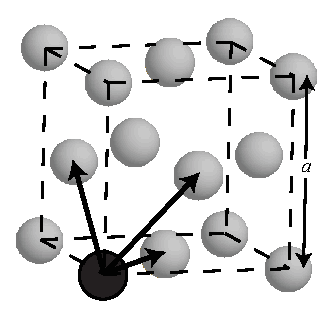
\includegraphics{/home/jason/thesis/thesis/table3-unitcell1.eps} 
% & Conventional (four atoms) 
% \newline 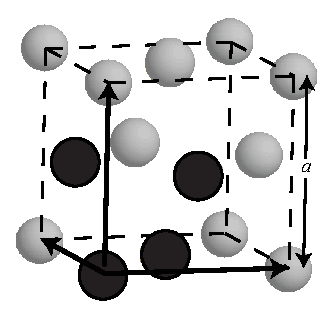
\includegraphics{/home/jason/thesis/thesis/table3-unitcell4.eps}\\ 
% \hline
% Basis& Face-centered Cubic & Simple Cubic\\ \hline
% Lattice Vectors& ($a/2$, $a/2$, 0), \newline ($a/2$, 0, $a/2$), 
% \newline (0, $a/2$, $a/2$)& ($a$, 0, 0), \newline (0, $a$, 0), 
% \newline (0, 0, $a$)\\ \hline
% Brillouin Zone& Truncated Octahedron \newline 
% 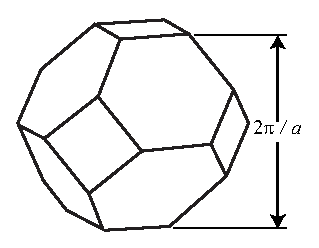
\includegraphics{/home/jason/thesis/thesis/table3-bz1.eps} & Cube \newline 
% 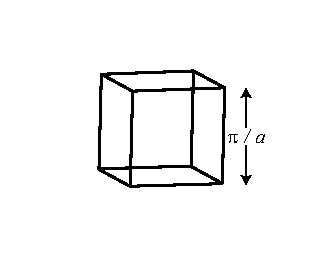
\includegraphics{/home/jason/thesis/thesis/table3-bz4.eps}\\ \hline
% Number of \newline Wave Vectors& $N$ & $N/4$\\ \hline
% Polarizations/\newline Wave Vector& 3 & 12\\ \hline
% \hline
% \end{tabular}
% \end{center}
% \caption{The unit cell for a face-centered cubic crystal can be chosen 
% in different ways.}
% \label{T-unitcell}
% \end{table}
% \renewcommand{\baselinestretch}{2.0}
% %--------------------------------------------------------------------------
% 
% \clearpage
% 
% The selection of the unit cell sets the shape of the Brillouin zone and 
% the points that will be resolved inside it (i.e., the allowed wave 
% vectors, $\pmb{\kappa}$). For a simulation cell with $N$ atoms, there 
% are $3N$ normal modes. If the unit cell has one atom, there will be $N$ 
% allowed wave vectors, each with three polarizations (i.e., dispersion 
% branches, which we will denote by $\nu$). For a four-atom unit cell, 
% there will be $N/4$ allowed wave vectors, each with 12 polarizations. 
% In general, the choice of an $n$-atom unit cell will lead to $N/n$ 
% allowed wave vectors, each with 3$n$ polarizations. As such, there are 
% always $3N$ normal modes.
% 
% %--------------------------------------------------------------------------
% \subsection{\label{A:symmetry}Crystal Symmetries (WORK)}
% %--------------------------------------------------------------------------
% 
% Symmetry operations define the properties of a crystal. 
% This applies to any vector or tensor property of the crystal. The 
% symmetries do not depend on the unit cell represenation, although 
% conventional unit cells may have additional symmetries compared 
% to the primitive unit cells which is due to the redundant information of 
% using a conventional cell. 
% 
% Ab initio codes such as abinit and quantum espresso also print the 
% symmetry operations information. The 
% \href{http://spglib.sourceforge.net/}{spglib} 
% package contains a library of routines for utilizing the 
% symmetry operations of.
% 
% Contact Ankit Jain for more information on symmetry operations 
% and their application to thermal transport calculations. 
% 
% For the crystalline systems studied in Section , the wavevectors 
% are averaged over according to their symmetries, 
% which reduces the list of wavevectors to the first octant of the 
% cubic BZ.\cite{mcgaughey_phonon_2004} This reduction is equivalent 
% to applying roations of the 
% \href{http://en.wikipedia.org/wiki/Rotation_group_SO(3)}
% {SO(3) Group}, or the group of 90 degree rotations in Euclidean 
% (3-dimensional) space. 
% Any succesive combination of 90 degree roations is also a symmetry 
% operation. This property leads to the identity
% \begin{equation}\label{EQ:kpt_sym}
%  \begin{split}
%   \pmb{\kappa} = -\pmb{\kappa},
%  \end{split}
% \end{equation}
% which is the application of two 90 degree rotations, and is a 
% \href{http://en.wikipedia.org/wiki/Parity_(physics)#Odd}
% {general property of any crystal}. 
% 
% \href{https://github.com/jasonlarkin/disorder/blob/master/matlab/issym.m}
% {Here is a matlab function} which compares two vectors 
% and checks if they are related by any number of orthogonal 
% rotations.
% 
% For the LJ argon example, further reduction  of the wavectors is 
% possible by using all symmetry 
% \href{http://spglib.sourceforge.net/#rotation}{rotation operations} 
% of the 
% \href{http://www.wolframalpha.com/input/?i=face-centered+cubic}
% {face centered cubic lattice}. Additional 
% \href{http://en.wikipedia.org/wiki/Translational_symmetry}
% {translational symmetry operations} may exist. 
% For example, for the cubic conventional cell of LJ argon, translational 
% symmetries ensure that all four atoms in the unit cell are 
% equivalent. Thus, the conventional cell has more total 
% symmetries (rotational plus translational) than the primitive cell, 
% which is due to the redundant information contained within it. Similar 
% to conventional unit cells, crystalline supercells also have a larger 
% number of translational symmetries.
% 
% %--------------------------------------------------------------------------
% \subsection{\label{A:unitcell}Primitive, Conventional, and Supercell 
% Representations using Normal Mode Decomposition (WORK)}
% %--------------------------------------------------------------------------
% 
% Having described the normal mode decomposition theoretical approach and 
% computational methodology in Sections \ref{S-NMDformulation} and 
% \ref{S-workflow}, we now carry out a case study on a LJ crystal at a 
% dimensionless temperature of 0.0827 (corresponding to an argon 
% temperature of 10 K). While this temperature is low (the LJ argon Debye 
% temperature is around 85 K), it will allow for a clean demonstration of 
% the technique. The LJ interatomic potential is computationally inexpensive 
% and is thus ideal for use in code development and testing. All results 
% will be presented in dimensionless LJ units \cite{ashcroft_solid_1976}. 
% The zero pressure lattice constant is 1.556 (Ref. 
% \citenum{mcgaughey_phonon_2004}) 
% and the potential energy is cutoff and shifted at a distance of 2.5.
% 
% From the same simulation cell and atomic data, one can perform normal 
% mode decomposition on either the primitive or conventional unit cells.
% \footnote{The allowed wave vectors are defined by the basis
% and the supercell used to perform the MD simulations. For a supercell 
% built using the conventional unit cell, as we use, the allowed wave 
% vectors can be labeled using either the conventional or primitive unit 
% cell description.  For a supercell built using the primitive unit cell, 
% however, all wave vectors cannot be labeled using the conventional unit 
% cell description.} The [100] and [111] dispersion curves and density of 
% states obtained from harmonic lattice dynamics calculations are plotted 
% for each unit cell in Figs. \ref{F-dispersion}(a) and (b). While the 
% dispersion curves in each direction show similarities, they are 
% necessarily different due to the allowed wave vectors and shape of the 
% Brillouin zone (see Table \ref{T-unitcell}). The density of states, 
% however, are identical, as expected and required. We note that the 
% conventional unit cell description leads to what appear to be optical 
% modes. In reality, these modes are a result of zone folding and can be 
% mapped directly to acoustic modes in the primitive unit cell description.
% 
% The MD simulations are run in the $NVE$ ensemble, the dimensionless 
% time step is 0.002, and the equations of motion are integrated using 
% the velocity Verlet algorithm. The system is equilibrated for $2^{20}$ 
% time steps before collecting data every 25 time steps for an additional 
% $2^{20}$ time steps. In order to capture system-size effects, cubic 
% simulation cells with between 256 and 6912 atoms are considered 
% (corresponding to between four and twelve conventional unit cells, $N_0$, 
% in each of the $x$, $y$, and $z$ directions). Ten simulations are 
% performed with different initial velocities and the autocorrelations 
% (or Fourier transforms) are averaged over the initial conditions and 
% symmetric wave vectors before fitting the phonon properties.
% 
% \vspace{10mm}
% %\clearpage
% 
% \begin{figure}[t]
% \begin{center}
% \includegraphics[scale=1]
% {/home/jason/Dropbox/book/m_book_lj_disp_dos_vg_prim_novg-2.eps}
% \includegraphics[scale=1]
% {/home/jason/Dropbox/book/m_book_lj_disp_dos_vg_conv_novg-2.eps}
% \caption{\label{F-dispersion} {Dispersion curves and full Brillouin zone 
% density of states for a LJ crystal at a dimensionless temperature of 
% 0.0827. (a) [100] and [111] dispersion curves and density of states 
% based on the primitive (i.e., one atom) unit cell. (b) [100] and [111] 
% dispersion curves and density of states based on the conventional (i.e., 
% four atom) unit cell. The harmonic lattice dynamics calculations are 
% performed using a resolution of sixteen wave vectors along the reciprocal 
% lattice vectors of the conventional unit cell. The red and blue dots in 
% (b) are the modes considered in Fig. \ref{F-bulkfitting}.}}
% \end{center}\normalsize
% \vspace*{-0mm}
% \end{figure}
% 
% \vspace{10mm}
% \clearpage
% 
% The lifetimes predicted from the frequency-domain analysis for the 
% primitive and conventional unit cell representations of the $N_0=10$ 
% system are plotted in Fig. \ref{F-bulklifetimes}(a). The difference 
% between the lifetimes is less than 5\%, which is within the uncertainty 
% of the fitting. A $1/\omega^2$ scaling, predicted from theory for 
% phonon-phonon scattering at low frequencies \cite{callaway_model_1959}, 
% is plotted and is in good agreement with the trend in the data at low 
% frequencies. Also plotted is the Ioffe-Regel (IR) limit 
% \cite{taraskin_determination_1999},
% \begin{eqnarray}
% \tau_{IR} = \f{2 \pi}{\omega},
% \end{eqnarray}
% which corresponds to when the phonon lifetime is equal to its period. 
% All the modes in the perfect system have lifetimes well above this limit. 
% It is interesting to note that the phonon lifetimes do not decrease 
% monotonically with increasing frequency, with a maximum observed near 
% $\omega = 18$. Such a maximum is also observed in silicon lifetimes 
% obtained from the SW potential \cite{turney_-plane_2010} and from DFT 
% calculations \cite{esfarjani_heat_2011}.
% 
% \begin{figure}[t]
% \begin{center}
% \includegraphics[scale=1]
% {/home/jason/Dropbox/book/m_book_lj_nmd_prim_conv_compare-2.eps}
% \caption{\label{F-bulklifetimes} Lennard-Jones lifetimes from a 
% $N_0=10$ system at a temperature of 0.0827 predicted from normal mode 
% decomposition analysis on (a) the primitive and conventional unit 
% cells, and (b) treating the simulation cell as the unit cell (i.e., 
% Gamma-point analysis). All lifetimes extracted from time-domain analysis.}
% \end{center}\normalsize
% \end{figure}
% 
% \clearpage
% 
% In performing the normal mode decomposition, one is not limited to the 
% primitive or conventional unit cells. As needed for disordered systems 
% (see Sections \ref{S-alloy} and \ref{S-amorphous}) one can define the 
% simulation cell as the unit cell, such that all normal modes have 
% $\pmb{\kappa}=\mathbf{0}$ (i.e., they are all at the Gamma-point).
% \footnote{In Gamma-point analysis, all normal modes have zero group 
% velocity and it is not possible to predict mean free paths or thermal 
% conductivity.} The lifetimes for Gamma-point analysis for the same MD 
% data used to generate the lifetimes in Fig.\ref{F-bulklifetimes}(a)   
% are plotted in Fig.\ref{F-bulklifetimes}(b). The trends for the 
% Gamma-point analysis are the same as for the primitive and conventional 
% unit cells. There is more scatter in the Gamma-point data as wave 
% vector symmetry averaging is no longer possible.
% 
% The phonon properties obtained from normal mode decomposition and 
% harmonic lattice dynamics calculations can now be used to predict bulk 
% thermal conductivity using Eq.\eqref{E-kBTE}. For classical MD 
% simulations the assumption of equipartition of energy is very good and 
% we take the volumetric specific heat to be $k_\mathrm{B}/V$ for all 
% modes \cite{mcgaughey_quantitative_2004,goicochea_thermal_2010,
% larkin_comparison_2012}.
% 
% The Gamma point corresponds to bulk translation and therefore does not 
% contribute to thermal conductivity. By discretizing the Brillouin zone, 
% we assign a volume to the Gamma point. The zero contribution of this 
% volume to the thermal conductivity introduces a size effect in the 
% prediction. To predict a bulk thermal conductivity, an extrapolation 
% procedure is used, whereby $k$ is plotted versus $1/N_o$ and a line is 
% fit to the data. The point on this line where $1/N_o=0$ gives the bulk 
% thermal conductivity \cite{turney_predicting_2009,esfarjani_heat_2011}. 
% This extrapolation 
% procedure requires that the low-frequency modes be dominated by
% intrinsic scattering (i.e., $\tau \propto \omega^{-2}$) and have a 
% similar group velocity \cite{shiomi_thermal_2011,esfarjani_heat_2011}. 
% For the LJcrystal, this requirement is satisfied for modest system sizes
% ($N_0 \ge 6$). The size-dependent and extrapolated thermal conductivities 
% are plotted in Fig.\ref{F-bulksizeeffect} for both the primitive and 
% conventional unit cells. The Green-Kubo predictions for the same system 
% are also plotted and show no size effect, consistent with previous work 
% \cite{mcgaughey_quantitative_2004}.
% 
% % \begin{figure}[t]
% % \begin{center}
% % \includegraphics[scale=1.0]
% % {/home/jason/Dropbox/book/m_book_cond_extrap_c0-3_boxon.eps}
% % \caption{\label{F-bulksizeeffect} Size dependence of thermal conductivity 
% % for the LJ crystal at a temperature of 0.0827 from normal mode 
% % decomposition and the Green-Kubo method.}
% % \end{center}\normalsize
% % \vspace*{-0mm}
% % \end{figure}
% 
% The extrapolated thermal conductivities from the primitive and 
% conventional unit cells are $177 \pm 15$ and $176 \pm 14$ W/m-K. 
% The Green-Kubo thermal conductivity is $173 \pm 13$ W/m-K. All thermal 
% conductivities agree well within their respective uncertainties.
% 
% For the perfect LJ crystal, there is no clear advantage of performing 
% the analysis in the time or frequency domains or for the primitive or 
% conventional unit cells. Challenges may emerge for high thermal 
% conductivity materials like silicon or carbon nanotubes, where the 
% time-domain decay may not be well described by an exponential and the 
% peaks in frequency space get narrow or are not well-fit by a Lorentzian. 
% The failure of the fitting for a perfect crystal is an indication that 
% the relaxation time approximation may not be appropriate and that care 
% should be taken when interpreting the results. In general, new materials 
% should be investigated on a case-by-case basis to determine the approach 
% that minimizes the uncertainty.

%--------------------------------------------------------------------------
\section{\label{A:NMD XCORR}NMD using Non-Exact Normal Modes}
%--------------------------------------------------------------------------

In Chapter \ref{Chapter:SED}, it was shown how NMD is 
applied to a perfect crystal. In reality, any crystal will have some 
deviation from perfect periodicity, which may be caused by a point defect, 
a dislocation, a grain boundary, or a free surface. In extreme cases, 
these deviations from periodicity will lead to the emergence of modified 
normal modes. For small perturbations, however, it is reasonable to
assume that the frequencies and mode shapes of the normal modes will 
be unchanged and that the effect of the perturbation will be on the 
lifetimes. Under this assumption, one can still project the atomic 
positions and velocities onto the normal modes of the unperturbed system.

While one could perform the NMD by projecting 
the atomic positions and velocities onto the modes of the unperturbed 
system, it is more appropriate to use the virtual crystal approximation 
(Section \ref{S:From VC Gamma}). 
Under the virtual 
crystal approximation, the system is replaced by one where all atoms 
have the same mass, equal to the average of the atomic masses in the 
system of interest. This system will have the same mode shapes as the 
original system, but the frequencies are modified due to the change 
in the average atomic mass.

Results for the time- and frequency domain approaches to NMD 
are shown for two modes for crystalline and alloyed LJ argon in 
Figs. \ref{F-alloyfitting}(a)-(d). These two modes are equivalent to 
those shown in the perfect crystal in 
Figs. \ref{F-dispersion}(b), \ref{F-bulkfitting}(a), and 
\ref{F-bulkfitting}(b). For a concentration, $c$, of 0.05, both peaks 
in the frequency domain are well-formed and a lifetime can be extracted 
by fitting the data to a Lorentzian function. This behavior is typical 
of all modes at a concentration of 0.05. The downward frequency shift 
is related to the increased average atomic mass.

For an alloy concentration of 0.5, the lower frequency mode still has 
a well-formed peak. The higher-frequency mode does not, however, such 
that a lifetime cannot be extracted by fitting to a Lorentzian function. 
Such behavior is typical of the higher frequency modes at high alloy 
concentrations. This change in behavior is also seen in the time domain, 
where the decay of the autocorrelation of the total mode energy is no 
longer a smooth exponential function. This behavior indicates that the 
virtual crystal normal mode is not a good description of the true 
normal mode. Equation \eqref{E:tau_E_xcorr} can be used to approximate a 
lifetime, as shown in Figs. \ref{F-alloyfitting}(c) and 
\ref{F-alloyfitting}(d).

These artifacts observed using NMD method with the virtual crystal 
approximation are not surprising given two considerations: 
(i) the MD simulations 
contain explicit disorder that influences the atomic trajectories, 
and (ii) the VC-normal modes are not the exact normal modes of the 
explicitly-disordered lattice supercells. 
An effective lifetime can be predicted 
using Eq. \eqref{E:tau_E_xcorr} 
because the VC total mode energy autocorrelations 
still decay to zero in a finite time. This result is to be expected 
given that the atomic trajectories contain 
information about the lattice energy, which from general statistical 
physics principles will have exponential relaxation behavior in an 
equilibrium ensemble.
\cite{landau_statistical_1980,srivastava_physics_1990,
rajabpour_thermal_2010} The lifetimes predicted from the VC-NMD method 
are in reasonable agreement with those predicted from the Gamma-NMD 
method, which uses the exact normal modes of the disordered supercell 
(Section \ref{S:From VC Gamma}).  

% For a normal mode of the lattice supercell 
% used for the MD simulations (i.e., a Gamma mode), 
% the total energy autocorrelation is an exponential function  
% with a decay time $\tau\kv$ and the kinetic energy autocorrelation is a 
% exponentially-damped sinusoidal oscillation with frequency 
% $2\omega\kv$ (see Section \ref{S:Subsection_SED_time-domain}). 
% When projecting MD simulations  
% of the explicitly disordered lattice supercells 
% onto the VC normal modes, 
% the energy autocorrelation functions 
% do not always follow these simple functional forms, 
% as shown in Fig. \ref{F:NMD XCORR} for two modes in the LJ alloy at a 
% concentration of 0.5.  
% By calculating the mode kinetic energy in the  
% frequency-domain, $\Phi$,\cite{larkin_comparison_2012} artifacts such as 
% multiple peaks are observed (see main plot).   



% %--------------------------------------------------------------------------
% \begin{figure}
% \begin{center}
% \includegraphics[scale=1.0]
% {/home/jason/disorder/paper/vc/fig10.eps}
% \vspace*{-5mm}
% \end{center}
% \caption{\label{F:NMD XCORR} The normal mode kinetic energy, $\Phi$,  
% of two modes (A and B) at wavevector [0.25 0 0] calculated 
% using VC-NMD for a mass disordered LJ FCC supercell 
% ($N_0=8$ and $c=0.5$) is shown in the main figure. 
% The VC dispersion-predicted peaks are labeled 
% by $\omega_0$. The inset shows the same mode's energy 
% [kinetic ($KE$) and total ($TE$)] autocorrelation functions.  
% Note the additional oscillation effects in the KE and TE autocorrelation 
% functions for Mode B which are due to the two peaks in $\Phi$. 
% A mode lifetime can 
% be extracted unambiguously using the integral of the TE autocorrelation 
% function [Eq. \eqref{EQ:tau_nmd} in Section \ref{S:From VC Gamma}].}
% \end{figure}
% %--------------------------------------------------------------------------

%--------------------------------------------------------------------------
\begin{figure}[t]
\begin{center}
\includegraphics[scale=1]
{/home/jason/Dropbox/book/m_book_lj_disp_dos_vg_prim_novg-2.eps}
\includegraphics[scale=1]
{/home/jason/Dropbox/book/m_book_lj_disp_dos_vg_conv_novg-2.eps}
\caption{\label{F-dispersion} {Dispersion curves and full Brillouin zone 
density of states for a LJ crystal at a temperature of 
10 K. (a) [100] and [111] dispersion curves and density of states 
based on the primitive (i.e., one atom) unit cell. (b) [100] and [111] 
dispersion curves and density of states based on the conventional (i.e., 
four atom) unit cell. The harmonic lattice dynamics calculations are 
performed using a resolution of sixteen wave vectors along the reciprocal 
lattice vectors of the conventional unit cell. The red and blue dots in 
(b) are the modes considered in Fig. \ref{F-bulkfitting}.}}
\end{center}\normalsize
\vspace*{-0mm}
\end{figure}
%--------------------------------------------------------------------------

%--------------------------------------------------------------------------
\begin{figure}
\begin{center}
\includegraphics[scale=1.0]
{/home/jason/Dropbox/book/m_book_lj_nmd_xcorr_compare_c0_c05_c5_sed.eps}
\includegraphics[scale=1.0]
{/home/jason/Dropbox/book/m_book_lj_nmd_xcorr_compare_c5_xcorr.eps}
\end{center}
\caption{\label{F-alloyfitting} 
Virtual crystal (a) frequency-domain 
and (b) time-domain NMD analysis for two modes 
in LJ alloys with concentrations of 0.05 and 0.5. For modes that are 
not well-approximated by the virtual crystal modes, the lifetime can 
be approximated using Eq. \eqref{E:tau_E_xcorr}, as shown in (d).
}
\end{figure}
%--------------------------------------------------------------------------
\vspace{5mm}
\clearpage

%--------------------------------------------------------------------------
\section{\label{A:metastability}Effect of Metastability for 
Amorphous Solids on Normal Mode Decomposition}
%--------------------------------------------------------------------------

Amorphous materials may have many different atomic 
configurations with nearly equivalent potential energies, 
leading to potential metastability during MD simulations 
\cite{buchenau_structural_1988,feldman_numerical_1999,
durandurdu_<i>ab_2002,bernstein_structural_2006,he_heat_2011}. 
This meta-stability can 
cause errors when predicting vibrational lifetimes using NMD, 
which is demonstrated below. 

This case study is performed on an amorphous LJ system with 2048 atoms 
at a temperature of 5 K. 
The amorphous solid is generated by liquefying the 
crystal, instantaneously removing all kinetic energy, and then relaxing 
the structure (i.e., a melt-quench, Sections \ref{S:Calculation} 
and \ref{S:Sample}). 
The MD simulation parameters are the same as for the 
LJ crystal and alloy (Section \ref{S:Calculation}). 
The LJ 
amorphous phase is metastable at this temperature and intermittently 
moves between very similar low-energy states. Evidence for the 
metastability can be found by analyzing the time-histories of the atomic 
displacements. As such, NMD, which requires the 
average atomic positions, will be an approximation.

The time- and frequency-domain approaches to NMD 
are shown for two mode in the amorphous system in 
Figs. \ref{F-amorphousfitting}(a) and \ref{F-amorphousfitting}(b). 
Because the analysis is performed at the Gamma-point, the peaks are 
well formed, but they are not Lorentzian. 
The oscillations in the total energy 
correlation for the low frequency mode is a consequence of the 
metastability of the amorphous phase. As such, the lifetimes are extracted 
by using Eq. \eqref{E:tau_E_xcorr}, as shown in the inset to 
Fig. \ref{F-amorphousfitting}(b). 
The lifetimes for the amorphous system are plotted in 
Fig. \ref{F-amorphouslifetimes}. Compared to the crystal, the lifetimes 
show little frequency dependence and a significant number at low 
frequencies fall below the IR limit [Eq. \eqref{EQ:IR}]. This result 
seems to be a consequence of the metastability, since this behavior 
is not observed for the NMD-predicted lifetimes for a-SiO$_2$ and a-Si 
(Fig. \ref{FIG:Lifetimes}, Section \ref{S:Life}), 
which were both annealed carefully to remove metastability 
(Section \ref{S:Sample}). Annealing the amorphous LJ system at the 
temperature studied does not remove metastability and leads to 
re-crystallization if performed for a long enough time ($>$ 5 ns). 

\begin{figure}[t]
\begin{center}
\includegraphics[scale=0.85]
{/home/jason/Dropbox/book/m_nmd_xcorr_fit_lj_plot-2.eps}
\caption{\label{F-amorphousfitting} (a) Time-domain and (b) frequency 
domain NMD analysis for two modes in an amorphous 
LJ solid at a temperature of 10 K.}
\end{center}\normalsize
\vspace*{-5mm}
\end{figure}

\begin{figure}[h]
\begin{center}
\includegraphics[scale=0.85]
{/home/jason/Dropbox/book/m_lj_nmd_c0_amor_life.eps}
\caption{\label{F-amorphouslifetimes} Lifetimes predicted by normal 
mode decomposition for an amorphous LJ phase at a  
temperature of 5 K. The lifetimes for the crystal at a 
temperature of 10 K are provided for comparison.}
\end{center}\normalsize
\vspace*{-5mm}
\end{figure}

\clearpage

%--------------------------------------------------------------------------
\section{\label{Appendix_A:Finite}Finite Simulation-Size Scaling for 
Thermal Conductivity}
%--------------------------------------------------------------------------

The thermal conductivities predicted by the NMD ($\Phi$), 
$\Phi'$, 
VC-NMD, VC-ALD, and GK methods 
are system size-dependent [i.e., $k = k(N_0)$] for all lattices 
and amorphous materials methods except 
perfect LJ argon from GK\cite{mcgaughey_quantitative_2004} and 
a-SiO$_2$ (Section \ref{S:Bulk}). 
To predict a bulk thermal conductivity, $k_{bulk}$,  
a linear extrapolation procedure is 
used, whereby 
\begin{equation}\label{EQ:k0}
\frac{k(N_0)}{k_{bulk}} = 1 - \frac{c_0}{N_0},
\end{equation}
where $c_0$ is a constant \cite{turney_predicting_2009,
esfarjani_heat_2011,shiomi_thermal_2011,he_thermal_2011}. 
This procedure is necessary because the first 
Brillouin zone is only sampled at a finite number of points for a finite 
simulation size, with no contribution from the volume at its center. To 
predict a bulk thermal conductivity, it is important to sample points 
near the Brillouin zone center, where the modes can have large lifetimes 
and group velocities \cite{turney_predicting_2009,sellan_size_2010}. 

The thermal conductivity 
is predicted for varying system sizes and the bulk thermal conductivity 
is obtained by fitting Eq. \eqref{EQ:k0} to the data. 
For the NMD ($\Phi$), $\Phi'$, VC-NMD, and VC-ALD methods, 
the validity of Eq. \eqref{EQ:k0}  
requires that the low-frequency modes be dominated by 
phonon-phonon scattering (i.e., $\tau\ \propto \omega^{-2}$) and  
follow the Debye approximation 
with respect to the group velocity and DOS 
\cite{shiomi_thermal_2011,esfarjani_heat_2011}. For the LJ 
argon alloys, this requirement is satisfied for modest system sizes 
(for $N_0 = 6$ to $12$).


%--------------------------------------------------------------------------
% \begin{figure}
% \begin{center}
% \includegraphics[angle=0,width=80.0mm]
% {/home/jason/thesis/thesis/appendix/LJ_NMD_SED_COND_2.eps}
% \end{center}
% \caption{\label{F:LJ_COND} Thermal conductivity predictions for LJ argon 
% calculated using phonon lifetimes predicted by $\Phi$ and $\Phi'$. (a) 
% The finite simulation-size scaling extrapolation 
% \cite{turney_predicting_2009,he_thermal_2011} 
% is used to compare the results to bulk predictions made using the 
% Green-Kubo method. (b) The bulk results for $\Phi$ and Green-Kubo are 
% in good agreement temperatures of $20$ and $40$ K with those of other 
% atomistic simulation methods,\cite{turney_predicting_2009} while those 
% from $\Phi'$ differ (see Table \ref{T:cond_table}).}
% \end{figure}
%--------------------------------------------------------------------------
%\clearpage


% %--------------------------------------------------------------------------
% \section{\label{Appendix:AF}AF Calculations (WORK)}
% %--------------------------------------------------------------------------
% 
% 
% % https://github.com/jasonlarkin/disorder/blob/master/lj/alloy/af_di_compare_broadening.m
% 
% The AF theory suggests a broadening which is larger than the average 
% frequency spacing, $\delta_{avg}$. 
% 
% The role of energy broadening in MD simulations could be helpful. The 
% energy of a given mode is broadened for two reasons: 
% 
% 1) due to anharmonic interactions.
% 
% 2) due to disorder (i.e., phonon-defect scattering in alloys, 
% diffuson theory). 
% 
% The NMD-predicted lifetimes are predicted from MD simulations where 
% all scattering mechanisms are present. Based on the comparison 
% of NMD- and AF-predicted diffusivities in Fig. , a frequency-dependent 
% broadening may be necessary for the AF theory. The role of frequency 
% broadening needs further investigation. 
% 
% %--------------------------------------------------------------------------
% \subsection{\label{Appendix:AF:Physical}Physical Picture}
% %--------------------------------------------------------------------------
% 
% The AF theory makes the harmonic approximation. Physically, modes 
% couple by spatial and energetic (harmonic, elastic scattering) overlap.  
% The strength of the overlap is determined by how close the mode 
% energies (frequencies) are and how much the eigenvectors spatially overlap. 
% The two highest frequency modes of the LJ alloy at a concentration of 
% 0.5 (see Section , Fig. ) are shown in Fig. . The mode frequencies are 
% and . These modes are both highly localized locons, which is indicated 
% by the small amount of spatial overlap in the eigenvector components. Only 
% the two spatial-dimensional components of the total three 
% spatial-dimensional components of the eigenvectors are plotted. The 
% three dimensional atomic coordinates are plotted in two dimensions. 
% 
% %--------------------------------------------------------------------------
% \begin{figure}
% \begin{center}
% \includegraphics[angle=0,width=80.0mm]
% {/home/jason/disorder/lj/alloy/m_eig_3d_plot_lj_alloy_c5_mode11999_12000.eps}
% \end{center}
% \caption{\label{F:LJ_COND} Spatial components of the eigenvectors of two 
% locons. The spatial localization is evident from the small amount of 
% spaital overlap of the mode eigenvectors.}
% \end{figure}
% %--------------------------------------------------------------------------
% 
% \clearpage
% 
% %--------------------------------------------------------------------------
% \subsection{\label{Appendix:AF:Finite}Finite Size Effects}
% %--------------------------------------------------------------------------
% 
% 
% % Hi Julian,
% % 
% % No problem about the silence, I have been busy trying to wrap up my thesis and find a job!
% % 
% % So, here are the issues:
% % 
% % 1) On the journey back from the most recent trip I was reading though the draft
% % manuscript that you sent me & puzzling over the issue of the size / Lorentzian sensitivity
% % of the answers.
% % 
% % Yes, this is kind of a tricky part of the AF method.  It seems like this was never addressed in the 
% % main paper, they simply suggest using a broadening equal to the average frequency spacing,\cite{feldman_thermal_1993} 
% % which is continued in \cite{feldman_numerical_1999} and \cite{shenogin_thermal_2009}. 
% % It turns out that the frequency spacing \delta_{freq} is strongly freq dependent, especially at low frequencies where the modes 
% % are sparse. Here is a crude plot for an a-LJ sample:
% % 
% % https://github.com/jasonlarkin/disorder/blob/master/lj/alloy/af_di_dw_amor.png
% % 
% % This has different effects depending on the system.  
% % 
% % For LJ alloys, the k_{AF} is strongly system-size dependent:
% % 
% % https://github.com/jasonlarkin/disorder/blob/master/lj/alloy/af_k_kmax.png
% % 
% % This is due to the harmonic approximation used in the AF theory, which leads to a Rayleigh scaling of 
% % the low-freq modes, \tau\propto\omega^{-4}. Here is another crude plot, showing the \omega^{-4} scaling 
% % predicted
% % 
% % https://github.com/jasonlarkin/disorder/blob/master/lj/alloy/af_di_all.png
% % 
% % While a-LJ shows a dependence on the broadening,  (\bra{\delta}=x*\delta_{avg} in this figure). Amorphous LJ is equivalent to a disordered lattice with a large disorder parameter.\cite{beltukov_ioffe-regel_2013}
% % 
% % 
% % The effect on a-Si is more complicated. For broaden = \delta_{avg}, the diffusivities at low frequency 
% % have large fluctuations. No definitive scaling can be seen, there seems to be a mix of \omega^{-4} and \omega^{-2} scalings. 
% % 
% % By increasing the broadening, the low frequency scaling can be tuned to match \omega^{-2} or \omega^{-4}:
% % 
% % https://github.com/jasonlarkin/disorder/blob/master/si/amor/m_af_si_normand_N0_3.png
% % 
% % The low-frequecy fluctuations can be smoothed by increasing the broadening over a small range:
% % 
% % https://github.com/jasonlarkin/disorder/blob/master/si/amor/m_af_si_normand_N0_5.png
% % 
% % This exaplins why Shenogin et al.'s prediction of k_{AF} = 1.0 W/m-K for a 512 atom system:
% % 
% % https://github.com/jasonlarkin/disorder/blob/master/si/amor/m_af_feldman_shenogin_fabian.png
% % 
% % which is due to using a small broadening. 
% % 
% % 
% % 
% % 
% % 
% % 
% % 1) I'm not quite clear on is what the final result is for the K_ph contribution that has to be
% % added. I realise that this was an early draft since all the cross referencing etc wasn't 
% % finished, and so perhaps you have an updated version that might help?
% % 
% % Ya sorry, that was a pretty early draft.  Here is the one which is just about to be submitted:
% % 
% % https://github.com/jasonlarkin/disorder/raw/master/paper/mfp/prb_mfp_jl_081613.pdf
% 
% %--------------------------------------------------------------------------
% % \begin{figure}
% % \begin{center}
% % \includegraphics[bb=0 0 3cm 3cm]
% % {/home/jason/disorder/lj/alloy/af_di_all.png}
% % \end{center}
% % \caption{\label{F:LJ_COND} Spatial components of the eigenvectors of two 
% % locons. The spatial localization is evident from the small amount of 
% % spaital overlap of the mode eigenvectors.}
% % \end{figure}
% % %--------------------------------------------------------------------------
% % 
% % 
% % %--------------------------------------------------------------------------
% % \begin{figure}
% % \begin{center}
% % \includegraphics[bb=0 0 3cm 3cm]
% % {/home/jason/disorder/lj/alloy/af_di_dw_0.05.png}
% % \includegraphics[bb=0 0 3cm 3cm]
% % {/home/jason/disorder/lj/alloy/af_di_dw_amor.png}
% % \end{center}
% % \caption{\label{F:LJ_COND} Spatial components of the eigenvectors of two 
% % locons. The spatial localization is evident from the small amount of 
% % spaital overlap of the mode eigenvectors.}
% % \end{figure}
% % %--------------------------------------------------------------------------
% % 
% % %--------------------------------------------------------------------------
% % \begin{figure}
% % \begin{center}
% % \includegraphics[bb=0 0 3cm 3cm]
% % {/home/jason/disorder/lj/alloy/af_di_kappa(broaden).png}
% % \end{center}
% % \caption{\label{F:LJ_COND} Spatial components of the eigenvectors of two 
% % locons. The spatial localization is evident from the small amount of 
% % spaital overlap of the mode eigenvectors.}
% % \end{figure}
% % %--------------------------------------------------------------------------
% % 
% % %--------------------------------------------------------------------------
% % \begin{figure}
% % \begin{center}
% % \includegraphics[bb=0 0 3cm 3cm]
% % {/home/jason/disorder/lj/alloy/af_k_kmax.png}
% % \end{center}
% % \caption{\label{F:LJ_COND} Spatial components of the eigenvectors of two 
% % locons. The spatial localization is evident from the small amount of 
% % spaital overlap of the mode eigenvectors.}
% % \end{figure}
% %--------------------------------------------------------------------------



% %--------------------------------------------------------------------------
% \section{\label{Appendix:SF}Spectral Density of Disordered Modes (WORK)}
% %--------------------------------------------------------------------------
% 
% %--------------------------------------------------------------------------
% % \begin{figure}
% % \begin{center}
% % \includegraphics[bb=0 0 3cm 3cm]
% % {/home/jason/disorder/lj/alloy/dsf_alloy_0.5_mode100.png}
% % \includegraphics[bb=0 0 3cm 3cm]
% % {/home/jason/disorder/lj/alloy/dsf_alloy_0.5_mode3000.png}
% % \includegraphics[bb=0 0 3cm 3cm]
% % {/home/jason/disorder/lj/alloy/dsf_alloy_0.5_mode4000.png}
% % \end{center}
% % \caption{\label{F:LJ_COND} Spatial components of the eigenvectors of two 
% % locons. The spatial localization is evident from the small amount of 
% % spaital overlap of the mode eigenvectors.}
% % \end{figure}
% %--------------------------------------------------------------------------
% 
% 
% %--------------------------------------------------------------------------
% \section{\label{Appendix:Accum}Size-effects for Low-frequency Dominated 
% Materials (WORK)}
% %--------------------------------------------------------------------------
% 
% %--------------------------------------------------------------------------
% \begin{figure}
% \begin{center}
% \includegraphics[angle=0,width=80.0mm]
% {/home/jason/disorder/si/alloy/m_ald_taud_si_cond_N0_ald_gk_nmd.eps}
% \end{center}
% \caption{\label{F:LJ_COND} Spatial components of the eigenvectors of two 
% locons. The spatial localization is evident from the small amount of 
% spaital overlap of the mode eigenvectors.}
% \end{figure}
% %--------------------------------------------------------------------------
% 
% \clearpage
% 
% %--------------------------------------------------------------------------
% \section{\label{Appendix:Accum}Accumulation Functions in Alloys 
% (WORK)}
% %--------------------------------------------------------------------------
% 
% 
% %--------------------------------------------------------------------------
% \begin{figure}
% \begin{center}
% \includegraphics[angle=0,width=80.0mm]
% {/home/jason/disorder/lj/alloy/m_ald_taud_lj_kaccum.eps}
% \end{center}
% \caption{\label{F:LJ_COND} Spatial components of the eigenvectors of two 
% locons. The spatial localization is evident from the small amount of 
% spaital overlap of the mode eigenvectors.}
% \end{figure}
% %--------------------------------------------------------------------------
% 
% \clearpage
% 
% %--------------------------------------------------------------------------
% \begin{figure}
% \begin{center}
% \includegraphics[angle=0,width=80.0mm]
% {/home/jason/disorder/lj/alloy/xcorr_alloy_cum_cond.eps}
% \end{center}
% \caption{\label{F:LJ_COND} Spatial components of the eigenvectors of two 
% locons. The spatial localization is evident from the small amount of 
% spaital overlap of the mode eigenvectors.}
% \end{figure}
% %--------------------------------------------------------------------------
% 
% \clearpage
% 
% %--------------------------------------------------------------------------
% \begin{figure}
% \begin{center}
% \includegraphics[angle=0,width=80.0mm]
% {/home/jason/disorder/si/alloy/m_ald_taud_si_klambda.eps}
% \end{center}
% \caption{\label{F:LJ_COND} Spatial components of the eigenvectors of two 
% locons. The spatial localization is evident from the small amount of 
% spaital overlap of the mode eigenvectors.}
% \end{figure}
% %--------------------------------------------------------------------------
% 
% \clearpage
% 
% %--------------------------------------------------------------------------
% \begin{figure}
% \begin{center}
% \includegraphics[angle=0,width=80.0mm]
% {/home/jason/disorder/si/alloy/m_ald_taud_si_cond_N0_ald_gk_nmd.eps}
% \end{center}
% \caption{\label{F:LJ_COND} Spatial components of the eigenvectors of two 
% locons. The spatial localization is evident from the small amount of 
% spaital overlap of the mode eigenvectors.}
% \end{figure}
% %--------------------------------------------------------------------------
% 
% \clearpage


